\documentclass[a4paper,10pt]{scrreprt}
\usepackage[utf8]{inputenc}
\usepackage{minted}
\usepackage{ngerman}
\usepackage{color}
\usepackage{colortbl}
\usepackage[dvipsnames]{xcolor}
\usepackage{fancyhdr}
\usepackage{lastpage}
\usepackage{geometry}
\usepackage{graphics}
\usepackage[pdftex]{graphicx}
\usepackage{hyperref}

%\usepackage{setspace}
%\onehalfspacing      

\geometry{inner=2.5cm,outer=2.5cm,top=3cm,bottom=3cm}

\definecolor{shadecolor}{gray}{.92}

%%% Einrückabstand Absatz:
\parindent 0pt

%%% Kopf und Fußzeilen
\pagestyle{fancy}
\fancyhead{} % lösche Kopfzeile
\fancyhead[RO,LE]{Martin Steinbach}
\fancyhead[LO,RE]{Service und Security Monitoring}
\fancyfoot{} % lösche Fußzeile
%\fancyfoot[LE,RO]{\thepage \hspace*{0.1cm} von\hspace*{0.2cm}\pageref{LastPage}}
\fancyfoot[LE,RO]{\thepage}
\fancyfoot[LO,CE]{Seminar Aufbereitung und Auswertung komplexer Daten}
\fancyfoot[CO,RE]{}
\renewcommand{\headrulewidth}{0.4pt}
\renewcommand{\footrulewidth}{0.4pt}

\usepackage{hyperref}
\hypersetup{
	pdftitle={Service- and Security Monitoring },
	pdfauthor={Martin Steinbach},
	pdfkeywords={Seminar, Rostock, SoSe 2018, 2018},
	pdfsubject={Seminar Aufbereitung und Auswertung komplexer Daten},
	pdfcreator={Martin Steinbach},
	citecolor=blue,
	hypertexnames=false,
	%linktocpage,
	pdfpagelabels,
	plainpages=false,
	backref,
	urlcolor=blue,
	menucolor=red,
	linkcolor=black,
	colorlinks=true,
	bookmarksnumbered,
	%pdffitwindow
}
%url linebreak after -
\def\UrlBreaks{\do\/\do-}

%\renewcommand{\thesection}{\Roman{section}} 
%\renewcommand{\thesubsection}{\thesection.\Roman{subsection}}

\usemintedstyle{}

\title{Service and Security Monitoring}
\author{Martin Steinbach}

\date{\today}

\begin{document}
\thispagestyle{empty}
\setcounter{page}{1}
\pagenumbering{roman}
\begin{center}
  
  {\Large \textsc{Seminararbeit}
  
  \vspace{4.25cm}
  
  {\fontsize{22}{22}\selectfont Service und Security-Monitoring\\}
  \vspace{0.75cm}
  {\fontsize{20}{20}\selectfont Seminar:\\\vspace{0.2cm} Aufbereitung und Auswertung 
  komplexer Daten}
}
  
  \vspace{7.25cm}
  
  {\Large Martin Steinbach
    
    \vspace{.15cm}
    
    Juni 2018}
  
  \vspace{1.5cm}
  
  
  
\includegraphics[scale=0.5]{img/siegel}
  
  \vspace{0.5cm}
  
  \rule{.7\textwidth}{.40pt}
  
  \vspace{.5cm}
  
  {\large\textsc{universität Rostock}}
    
    \vspace{.15cm}
        
\end{center}
\quad  \addtocounter{page}{-1}
\newpage

\vspace*{\fill}
\textbf{Exzerpt}\\\\
    Servicemonitoring ist eine wichtige Voraussetzung um eine zuverlässige 
    IT-Infrastruktur zu betreiben. Monitoring ist auch geeigent um IT-Sicherheitskritische
    Ereignisse zu identifizieren und adäquat auf diese zu reagieren. Die Vorliegende
    Arbeit bietet eine Einführung in die Thematik der Dienstüberwachung und stellt die
    beiden Überwachungsformen Aktive- und Passive-Überwachung vor. Es wird zudem
    die Frage geklärt, warum Servicemonitoring auch gleichzeitig Securitymonitoring ist.
    Anschließend wird anhand eines existierenden Prototypen aufgezeigt, wie eine 
    Korrelation von Ereignissen in Cloud-Umgebungen realisiert werden kann. In Abschnitt 
    drei wird eine mögliche Visualisierungslösung für die korrelierten Daten vorgestellt. 
    Die letzte Sektion zieht ein Fazit und blickt zukünftige Ideen für die Entwicklung 
    des Prototypen. 
\vspace*{\fill}


\tableofcontents
\thispagestyle{fancy}
%%%%%%%%%%%%%%%%%%%%%%%%%%%%%%%%%%%%%%%%%%%%%%%%%%%%%%%%%%%%%%%%%%%%%%%
\cleardoubleemptypage
\setcounter{page}{1}
\pagenumbering{arabic}
\chapter{Einführung}\label{01_einf}
\thispagestyle{fancy}

In diesem Kapitel wird anhand der IT-Sicherheitsziele aufgezeigt, dass man unter dem 
Begriff Servicemonitoring auch immer den Begriff Securitymonitoring verstehen
kann. Auch soll darauf hingewiesen werden, dass der Ausdruck Überwachung im ganzen
Dokument mit der Bedeutung: Aufsicht oder Monitoring belegt wird um eine klare Abgrenzung
zur zweiten Bedeutung: Observation, Beschattung (engl. surveillance) zu erlangen.


\section{Servicemonitoring und Securitymonitoring}

Die Überwachung von Diensten ist mittlerweile ein integraler Bestandteil der 
Infrastruktur jedes IT-~Diensteanbieters geworden. Neben der einfachen Erfassung
und der (z.B. grafischen) Aufarbeitung verschiedenster Messgrößen, werden die erfassten 
Daten zunehmend analysiert und es wird versucht Muster zu erkennen. Dieser Vorgang wird 
auch als \textit{BigData} bezeichnet. Diese Daten werden auch verstärkt zur 
Sicherheitsanalyse herangezogen. Daher stellt sich die Frage, ob Securitymonitoring 
äquivalent zum Servicemonitoring - Begriff ist. Um es vorweg zunehmen, ja, denn es kommt 
ausschließlich auf die Fragestellung an, die man mit den erfassten Daten klären möchte. 
Im Folgenden werden die drei Hauptziele der IT-Sicherheit aufgeschlüsselt und in 
Beziehung mit dem Servicemonitoring - Begriff gebracht.\\\\

\underline{\textbf{Vertraulichkeit}}\\\\
Das Ziel der Vertraulichkeit sagt aus, dass der Zugriff auf Daten ausschließlich von
autorisierten Nutzern erfolgen darf, egal in welchem Modus. Erreicht wird das Ziel zum
Beispiel durch Zugriffsrechte, wie z.B. Mandatory Access Control (MAC) und 
\footnote{Zugriffkontrollstrategie aus systemweiten Regeln, 
bei der nicht nur die Nutzeridentität ein Rolle spielt.} oder Discretionary Access 
Control(DAC)\footnote{Zugriffskontrollstrategie, bei der lediglich nie Nutzeridentität 
eine Rolle spiel (übliches Rechtesystem).} und vor allem durch Verschlüsselung.\\

Die Frage, ob sich Vertraulichkeit überwachen lässt, ist nur teilweise beantwortbar.
Stellt man sich ein System vor auf dem ein nicht autorisierter Nutzer Zugriff auf
Informationen erlangt, so ist dies messbar und es ist möglich eine Meldung 
zu generieren (z.B. eine Log-Meldung oder eine Nachricht an Verantwortliche). Wird 
jedoch ein autorisiertes Konto durch einen nicht autorisierten Nutzer kompromittiert,
gestaltet sich die Entdeckung dieses Ereignisses schwieriger. Ob es sich in diesem Fall 
um einen erlaubten Zugriff des tatsächlichen Nutzers oder einen nicht erlaubten Zugriff
handelt kann nur unter der Zuhilfenahme weiterer Information geklärt werden.
Zum Beispiel könnte die Quelle (Kapitel \ref{ausblick}), von der aus sich der Nutzer 
Zugriff verschafft hat, miteinbezogen werden. Auch die Korrelation mit Zeitdaten, an 
denen sich der zugriffsberechtigte Nutzer einloggt, können zur Klärung hinzugezogen 
werden.\\\\

\underline{\textbf{Verfügbarkeit}}\\\\
Ob ein Dienst Verfügbar ist, wird dadurch geklärt, ob der Zugriff auf Informationen
innerhalb eines gewissen Zeitraums erfolgreich ist.\\

Die Verfügbarkeit gleicht damit auch der grundlegenden Fragestellung des 
Servicemonitorings. Ist ein gewisser Dienst erreichbar und ist dessen 
Abarbeitungsgeschwindigkeit in einem vorgegebenem Rahmen?\\\\
\newpage
\underline{\textbf{Integrität}}\\\\
Integrität wird erreicht, wenn eine Änderung der Daten nicht unbemerkt geschieht. Es soll 
somit ein Indikator für die Veränderung existieren. Um dieses Ziel zu erreichen werden
Verfahren wie digitale Signatur und Hashes verwendet.\\

Auch das Ziel der Integrität lässt sich kontrollieren, dazu finden die selben Maßnahmen 
Verwendung wie in der IT-Sicherheit. Es lassen sich zum Beispiel auf regelmäßiger Basis 
Daten prüfen, von denen man vorher mit einem kryptografisch sicheren Verfahren ein Hash 
errechnet hat. Ändert sich die Hashsumme, ohne das ein Zugriff auf die Daten genehmigt 
wurde, ist dies ein Integritätsverlust.\\

Zusammengefasst ist Monitoring von IT-Infrastruktur immer auch gleich Securitymonitoring. 
Mithilfe eines lückenlos ausgerollten Monitorings ist es demnach möglich einen Beweis zu 
führen, zu welchem Zeitpunkt ein gewisser Dienst welchen Zustand hatte.
 
\section{Motive}

Der Grund warum eine dauerhafte Überwachung von Infrastruktur und den darauf aufbauenden 
Diensten keine Option sondern obligatorisch sein sollte, ist recht simpel zu erörtern. 
Allein die in \cite[461]{francia} berichteten Zahlen sprechen für sich. $90\,\%$ aller 
Firmen waren schon Cyberattacken ausgesetzt, $80\,\%$ davon haben dadurch erhebliche 
finanzielle Einbußen erlitten. Aktuell werden innerhalb eines Jahres $86\,\%$ der großen 
nordamerikanischen Unternehmen Opfer von Cyberattacken und der Diebstahl des geistigen 
Eigentums hat sich in den Jahren 2011-2015 verdoppelt.\\
Auch der aktuelle, jährlich veröffentlichte Lagebericht zur nationalen IT-Sicherheit des
Bundesamtes für Sicherheit in Informationstechnik (BSI) \cite[12]{bsi-lagebericht} 
berichtet  
von einer Cyberattacke auf eine großen deutschen Industriekonzern. Etwa \textbf{zwei 
Monate} konnten unbemerkt Daten aus weltweit verteilten Standorten in Richtung 
Südostasien abfließen bevor der Vorfall detektiert wurde. Aus den Empfehlungen des BSI 
lässt sich schließen, dass neben einer ungünstigen Netzwerksegmentierung auch 
mangelhaftes Monitoring der Grund für die späte Erkennung war. In diesem Zusammenhang ist 
auch der Angriff auf den Deutschen Bundestag im Jahr 2015 erwähnenswert, da auch in 
diesem Fall einige Wochen lang unbemerkt Daten abfließen konnten und das Ziel 
hoheitliches war, Technologietransfer und finanzielle Absichten also eine untergeordnete 
Rolle gespielt haben.
%\newpage
\subsection{Behörden mit Überwachungsauftrag}

Aufgrund der zuvor dargestellten Gründe, wurden in den letzten Jahren eine Reihe an neuen 
Behörden in der Bundesrepublik Deutschland gegründet, deren Auftrag die Überwachung 
(Monitoring) wichtiger Infrastrukturen innerhalb der Grenzen der Bundesrepublik ist. Zum 
Einen das Nationale Cyber-Abwehrzentrum (NCAZ) \cite{web_ncaz} mit Sitz in Bonn. Die 
Aufgabe des NCAZ ist die Koordinierung von Abwehrmaßnahmen und Informationskonsolidierung 
über den Aufbau von rein ziviler Infrastruktur über mehrere Behörden hinweg. Das 
Nationale IT-Lagezentrum \cite{web_lagezentrum} überwacht hingegen aktiv die 
Regierungsnetze und erstellt monatliche Lageberichte. Auf militärischer Seite übernimmt 
der Bundeswehr-Organisationsbereich Cyber- und Informationsraum (CIR) diese Aufgabe.

\section{Überwachungsformen}

Es lassen sich zwei verschiedene Überwachungsformen identifizieren. Die aktive 
Überwachung, bei der aktiv Status und Messwerte von Diensten erfragt werden, sowie die 
passive Überwachung, bei der die Dienste selbstständig Meldungen an einen zentralen 
Punkt, den Monitor, senden. Unter einem Dienst wird in diesen Beispielen nicht nur ein 
\textit{service} oder \textit{daemon}\footnote{Bezeichnung eines Dienstes auf 
Unix-basierenden Systemen.} sondern jegliche Entität, deren Status Messbar ist, 
verstanden.

\subsection{Aktive Überwachung}
\begin{figure}[htbp]
    \caption{Sequenzdiagramm: Aktive Überwachung}
    \label{aktiv}\vspace{0.2cm}
    \centering
    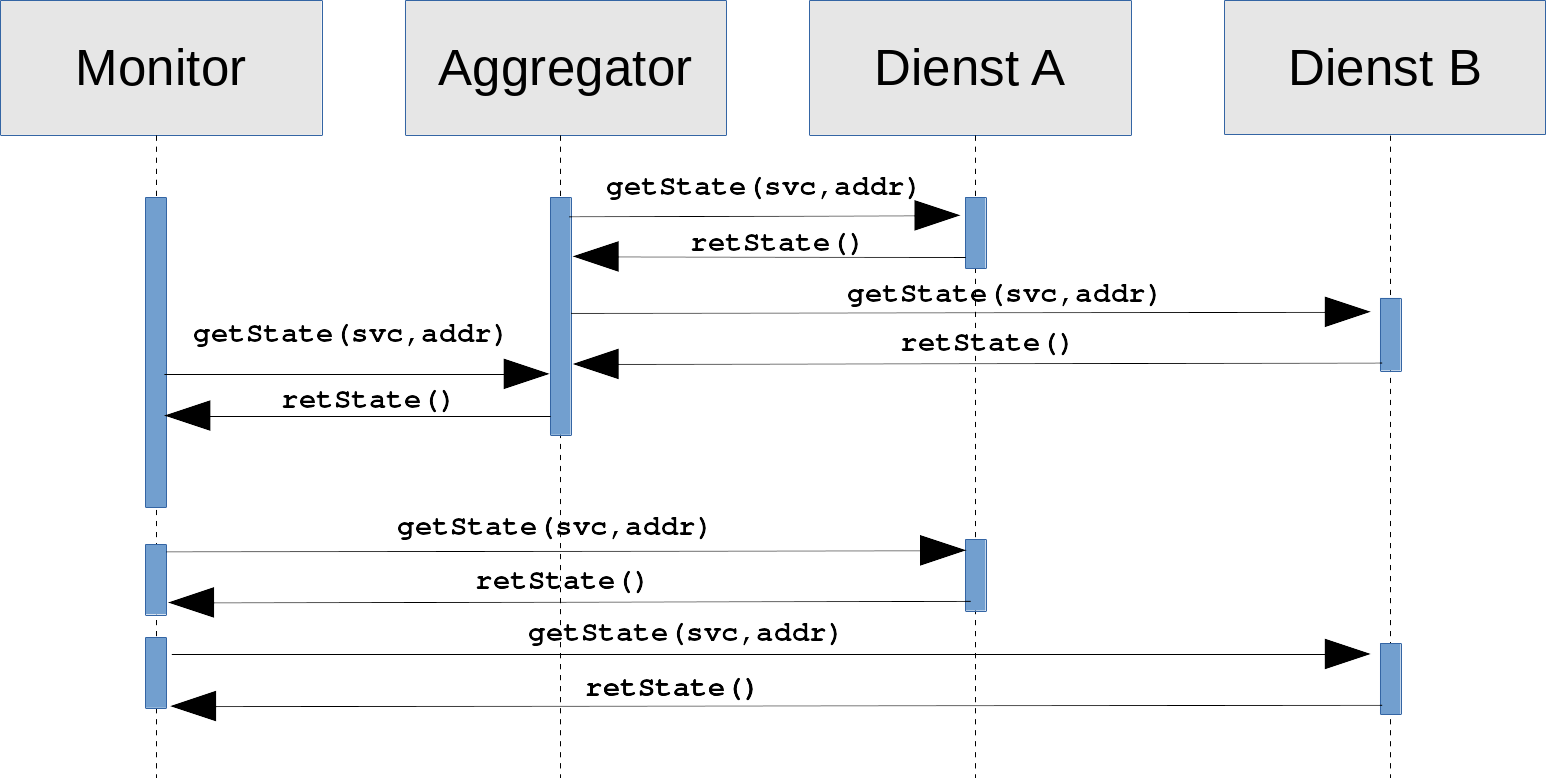
\includegraphics[scale=0.36]{img/sequence_uml_active_trans}

\end{figure}

Obiges Sequenzdiagramm (Abbildung \ref{aktiv}) zeigt schematisch den Ablauf von aktiver 
Überwachung. \emph{Monitor} ist die zentrale Instanz auf der alle zu überwachenden 
Informationen gesammelt, aufbereitet und ausgegeben werden. Jedoch muss der 
\emph{Monitor} nicht alle Information sammeln, es können auch hierarchisch untergeordnete 
\emph{Aggregatoren} existieren, welche ebenfalls Informationen von verschiedenen Diensten 
erheben. Diese \emph{Aggregatoren} können aus Leistungsgründen vor einen \emph{Monitor} 
geschaltet werden, um die Anzahl an abzufragenden Diensten für den \emph{Monitor} zu 
verringern. In diesem Fall bereitet bereits der \emph{Aggregator} die Daten auf und der 
\emph{Monitor} fragt nur noch die schon konsolidierten Informationen ab. Aber auch 
Segmentierungen von Infrastruktur können diesen Aufbau notwendig machen, wenn z.B. 
\emph{Monitor} \emph{Dienst A} und \emph{Dienst B} nicht direkt erreichen kann oder darf. 
Zur Klassifizierung von Ereignissen werden in Überwachungslösungen\footnote{zum Beispiel: 
Nagios, Icinga} oft verschiedene Status verwendet, dies dient hauptsächlich zum 
schnelleren Verständnis für die auswertende Person. Aus diesem Grund wurden in 
Abbildung \ref{aktiv} die Bezeichnungen für der Abfragefunktionen \texttt{getState()} und 
\texttt{reState()} gewählt. Mögliche Status für die Rückgabe sind in Tabelle 
\ref{table:status} aufgeführt.

\begin{table}[ht]
    \caption{Statusübersicht}
    \label{table:status}\vspace{0.2cm}
    \centering{
    \renewcommand{\arraystretch}{1.3}
    
    \begin{tabular}{|l|l|}
        
        \hline
       \rowcolor{gray!40} \textbf{Statusbezeichnung} & \textbf{Statusbeschreibung}\\
        \hline
        \texttt{OK} & Dienst läuft innerhalb normaler Parameter.\\
        \texttt{WARNING}& Die (zuvor definierte) Warnschwelle wurde überschritten.\\
        \texttt{CRITICAL}& Die kritische Schwelle wurde überschritten oder es gab einen
        Timeout.\\
        \texttt{UNKNOWN}& Ein undefinierter Wert wurde an \emph{Monitor} übermittelt.\\
        \hline
    \end{tabular}
}

\end{table}
Ein Visualisierungsbeispiel für einen Statusverlauf eines überwachten Dienstes befindet 
sich im Anhang (Abbildung \ref{app:nag}).

\newpage
Mithilfe der Techniken zur aktiven Überwachung lassen sich zwei Klassen überwachbarer 
Dienste identifizieren: Die Betriebssystemabhängigen und die Betriebssystemunabhängigen 
Dienste. Tabelle \ref{table:aktiv} listet einige Beispiele für die jeweilige Klasse auf.


     
\begin{table}[ht]
\caption{Beispiele für aktive Überwachung}
\label{table:aktiv}\vspace{0.2cm}
\centering{
\renewcommand{\arraystretch}{1.3}
\begin{tabular}{|l|l|}
    \hline
    \rowcolor{gray!40}\textbf{Dienst / Entität }& \textbf{Beispiel} \\
    \hline
    \multicolumn{2}{|l|}{\cellcolor{shadecolor}\textbf{Betriebssystemabhängig}}\\
    \hline
    Auslastung & wie viel CPU-Zeit benötigt ein bestimmter Prozess/das ganze System\\
    Speicher & Speicherauslastung des Systems/ Belegung persistenter Speicher\\
    Prozesse & läuft ein bestimmter Prozess/ wie viele Prozesse eines Namens laufen\\
    Datendurchsatz & wie viele Bytes passieren ein Interface, Anzahl an
    \emph{paket-drops},\emph{rejects}\\
    Audit & wurden Zugriffsregeln verletzt/ welcher Nutzer hat auf Datei X zugegriffen\\
    \hline
    \multicolumn{2}{|l|}{\cellcolor{shadecolor}\textbf{Betriebssystemunabhängig}}\\
    \hline
    \texttt{ICMP} & Netzwerkschnittstelle/ System erreichbar, \emph{round trip 
    time}\\
    \texttt{TCP/UDP} & ist bestimmter \emph{port} erreichbar\\
    Anwendungsprotokolle & Login möglich / Referenzdaten abrufbar / Rückgabewerte 
    Testroutinen\\
    \texttt{SNMP} & Abfrage beliebiger und 
    zum Teil standardisierter Messwerte\\
    \hline
\end{tabular}


}
\end{table}

\subsection{Passive Überwachung}
\begin{figure}[htbp]
    \caption{Passive Überwachung}
    \label{passiv}\vspace{0.2cm}
    \centering
    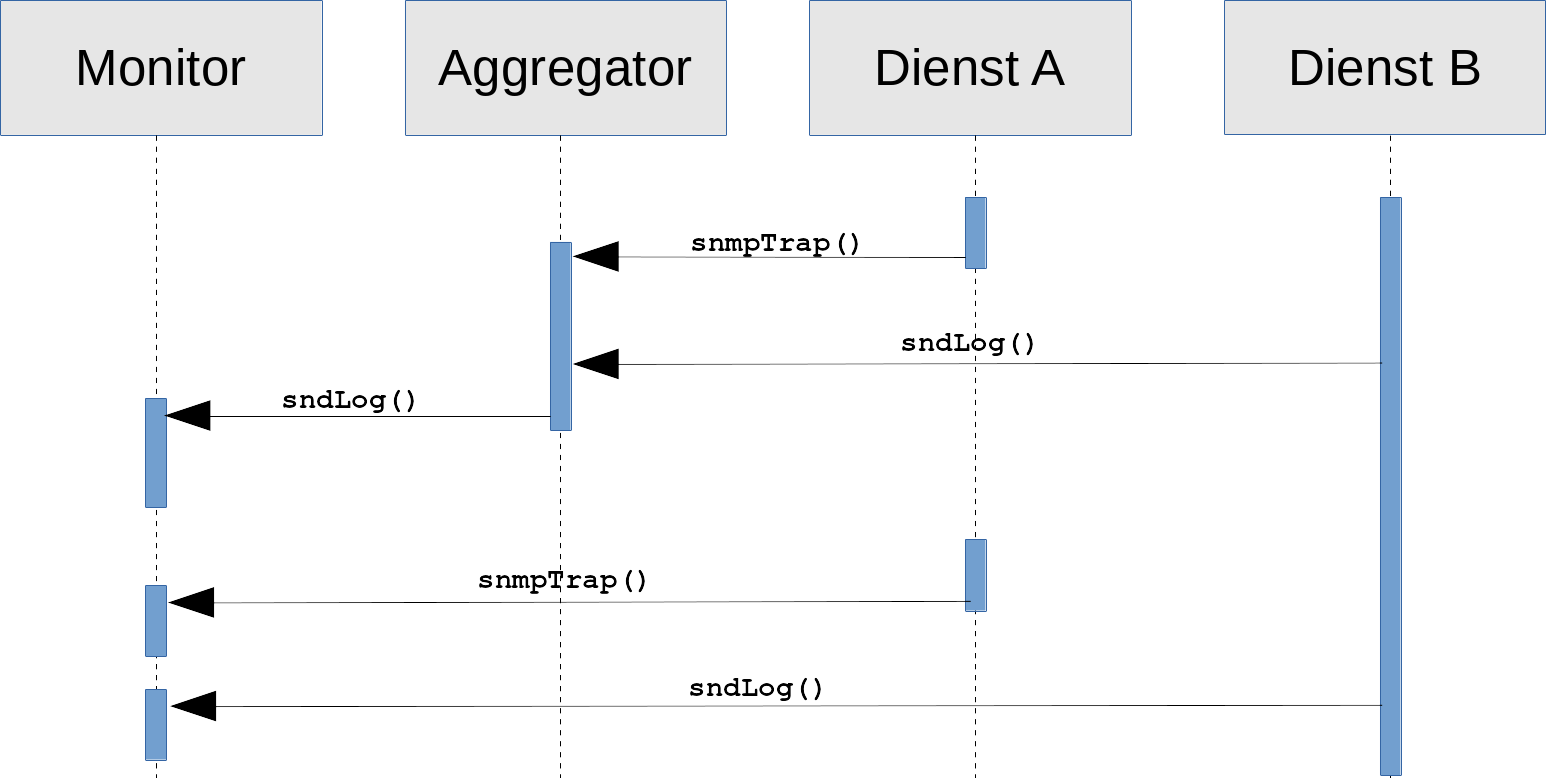
\includegraphics[scale=0.36]{img/sequence_uml_passive_trans}

\end{figure}

Wie in Abbildung \ref{passiv} zu erkennen, werden bei der passiven Überwachung nur Daten
ausgewertet, welche durch Dienste selbst generiert werden oder aber durch eine Software, 
welche den Dienst lokal überwacht. Es erfolgt keine Abfrage bei den Diensten. Der 
zentrale Punkt, welcher auch die Auswertung übernimmt, bleibt passiv und empfängt 
lediglich Meldungen. Am häufigsten sind diese Meldungen LOG-Meldungen, generiert von 
einem LOG-System. Aber auch SNMP\footnote{Simple Network Management Protocol: 
Ermöglicht eine plattformunabhängige Überwachung verschiedenster 
Endgeräte.}-Traps\footnote{SNMP-Trap: aktive Benachrichtigung des Monitors durch ein 
Endgerät/Dienst.} fallen unter diese Kategorie, daher auch die Wahl der 
Funktionsbezeichner in Abbildung \ref{passiv}.
%%%%%%%%%%%%%%%%%%%%%%%%%%%%%%%%%%%%%%%%%%%%%%%%%%%%%%%%%%%%%%%%%%%%%%%
\chapter{Logkorrelation in Cloud-Umgebungen}\label{02_jcorrelat}
\thispagestyle{fancy}

Im folgenden Abschnitt wird eine Forschungsarbeit der Fachhochschule Fulda 
\cite{reissmann} vorgestellt. Ziel der Forschung war und ist es, ein gut skalierendes 
System zu entwickeln um eine automatisierte Auswertung von Syslog-Meldungen in 
Cloud-Umgebungen bereit zu stellen. Aufgrund der enormen Datenmengen die in solchen 
Umgebungen anfallen kann eine Auswertung nur mittels korrelations- und 
Aggregationsverfahren geschehen. Um dieses Ziel zu erreichen kommen verschiedene 
Standards und eine Reihe von Software-Lösungen zum Einsatz.

Nachfolgend werden einige wichtige Begriffe geklärt, die Anforderungen identifiziert, die 
verwendeten Standards und die eingesetzte Software erläutert und im Weiteren Verlauf des 
Abschnitts wird anhand eines Beispiels eine Syslog-Korrelation vorgenommen.

\section{Anforderungen}\label{anforderungen}

Viele Unternehmen haben in den letzten Jahren einen großen Teil ihrer IT-Infrastruktur 
ausgelagert. Laut Analysen werden bis 2025 80 \% aller Unternehmen \cite{web_ix} 
weltweit ihre eigene Rechenzentrumsinfrastruktur abgeschaltet haben. Die wenigen Anbieter 
von Cloud-Infrastruktur stehen in Konkurrenz miteinander, daher existieren auch keine 
einheitlichen Schnittstellen um auf die Cloud-Konfigurationen zuzugreifen. Für die 
Überwachung, speziell von Sicherheitskritischen Ereignissen, stehen ebenso nur 
proprietäre Schnittstellen jedes Anbieters zur Verfügung. Aus diesem Grund soll ein 
System geschaffen werden, das die gewaltige Menge an aufkommenden Logdaten, unabhängig 
vom Anbieter, analysiert und sicherheitskritische Ereignisse unverzüglich zu 
identifiziert. Insbesondere soll das System das dynamisch sinkende und wachsende 
Syslog-Aufkommen beherrschen können. Denn durch die fluide Kostenstruktur der 
Cloud-Anbieter können schnell neue virtuelle Maschinen erstellt und entfernt werden, je 
nachdem wie viel Leistung der Kunde gerade benötigt.
Darüber hinaus sollen Meldungen auch persistent gespeichert werden, vornehmlich zur 
Erstellung von Trends und Langzeitanalysen, dabei soll der benötigte Speicherplatz so 
gering wie möglich gehalten werden.

\section{Beispielszenario}\label{szenario}

Im weiteren Verlauf dieses Kapitels soll zur detaillierteren Darstellung der 
Leistungsfähigkeit einer automatischen Syslog-Korrelation ein gängiges 
Angriffsszenario dienen. Eine \textit{ssh}-BruteForce Attacke auf eine beliebige Anzahl
an überwachten Systemen. Dabei soll genau der eine erfolgreiche Login innerhalb  der 
enormen Anzahl an erfolglosen oder ungültigen Versuchen identifiziert werden. Dieses 
recht einfache Szenario ist bei der erheblichen Anzahl an möglichen Systemen (10K+) 
manuell unmöglich zu bewerkstelligen.

\newpage
\section{JCorrelat}\label{sec_jcorrelat}

In Abbildung \ref{pic:jcorrelat} \cite[47]{reissmann} ist der schematische Aufbau von 
JCorrelat dargestellt, ein Prototyp der die Anforderungen aus Abschnitt 
\ref{anforderungen} erfüllen soll. Die hinzugefügten Nummern dienen der Übersichtlichkeit 
im weiteren Erklärungsverlauf.   

\begin{figure}[htbp]
    \caption{Aufbau von JCorrelat}
    \label{pic:jcorrelat}\vspace{0.2cm}
    \centering
    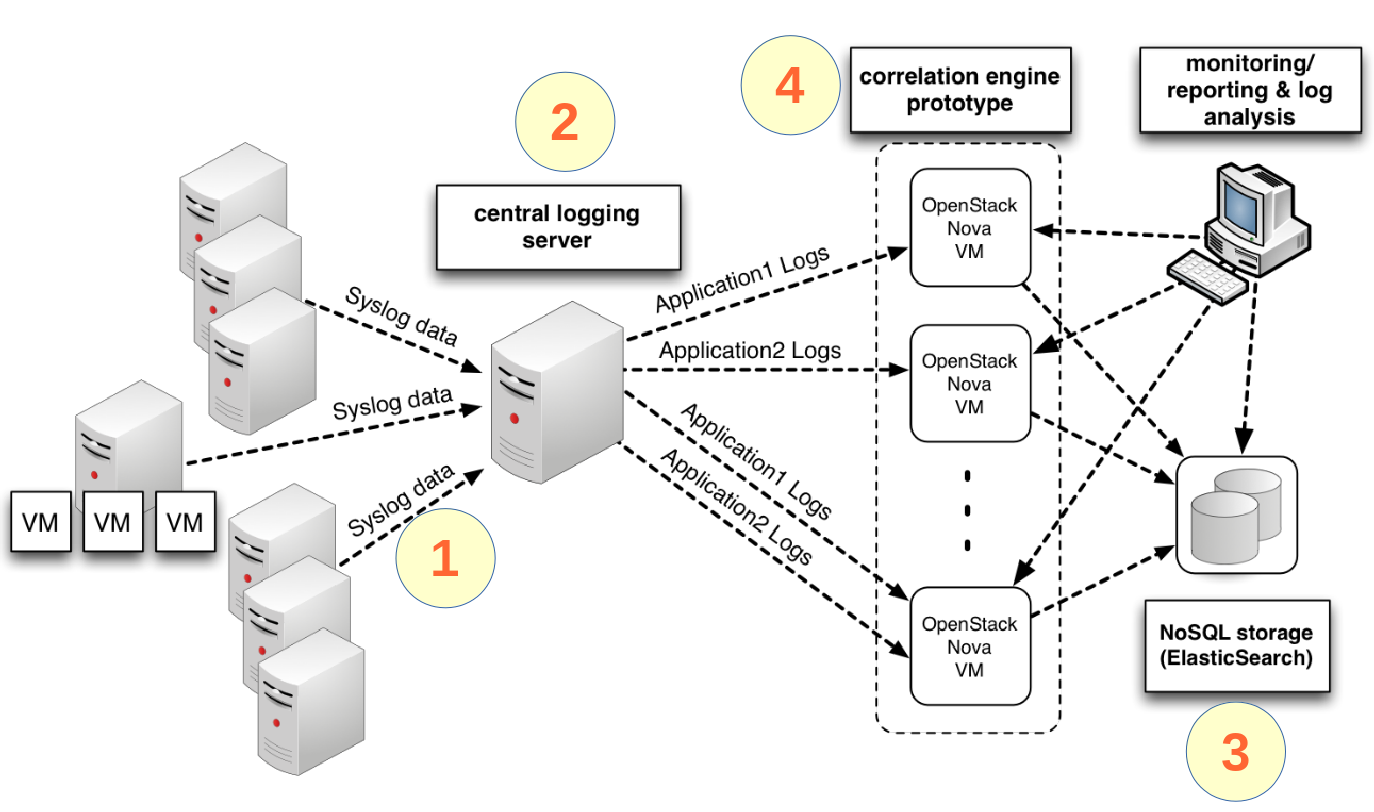
\includegraphics[scale=0.36]{img/schema-correlat}
    
\end{figure}

\subsection{Syslog-Protokoll} \label{syslog-proto}

Als Ereignisquelle und als Grundlage für neu generierte Meldungen wird das 
Syslog-Protokoll verwendet. Es ist das meist verbreitete Log-Format und wurde 
bereits in RFC 3164 standardisiert, jedoch sieht dieser Standard keine strukturierten 
Daten (\texttt{key $\Rightarrow$ value}) innerhalb einer Syslog-Nachricht vor. 
Erst mit RFC 5424 \cite{rfc5424} wurde diese Funktionalität hinzugefügt.

\begin{table}[ht]
    \caption{Aufbau RFC 5424}
    \label{table:rfc5424}\vspace{0.2cm}
    \centering{
        \renewcommand{\arraystretch}{1.3}
    \begin{tabular}{|l|c|c|}
        \hline 
        \rowcolor{gray!40} \textbf{Feld}&  \textbf{Inhalt}& \textbf{Beispiel}\\ 
        \hline
        \hline
         \multicolumn{3}{|l|}{\cellcolor{shadecolor}\textbf{HEADER}}\\
         \hline
         facility & $int \in \{0..23\}$  & $<$\textbf{16}5$>$ (\texttt{local0}) \\ 
        \hline 
        \rowcolor{green!15} severity & $ int \in \{0..7\}$  &$<$16\textbf{5}$>$  
        (\texttt{Notice})\\ 
        \hline
         timestamp & \texttt{RFC3339}  &\verb|2003-10-11T22:14:15.003Z|\\ 
        \hline 
         hostname & string  &\verb|mymachine.example.com|\\ 
        \hline 
        \rowcolor{green!15} tag &string  &\verb|evntslog|\\
        \hline
         \multicolumn{3}{|l|}{\cellcolor{shadecolor}\textbf{MESSAGE}}\\     
        \hline
         MSGID& string &\verb|ID47| \\
        \hline
        \rowcolor{green!15} structured data& key=value &\verb|eventID="1011"| \\
        \hline
         content &string&\verb|An application event log...| \\
        \hline
    \end{tabular} 
    }
\end{table}

\newpage

\begin{figure}[h]
    \caption{Beispiel RFC5424 Syslog-Meldung}
    \label{log_example}\vspace{0.2cm}
    \centering
    \begin{shaded*}
    \small{
        \begin{verbatim}
        
        
        <165> 2003-10-11T22:14:15.003Z mymachine.example.com evntslog - ID47 
        [exampleSDID@32473 iut="3" eventSource="Application" eventID="1011"] BOMAn 
        application event log entry...
        \end{verbatim}}
    \end{shaded*}
\end{figure}





Tabelle \ref{table:rfc5424} zeigt den Aufbau eines Syslog-Paketes nach RFC 5424 und 
Abbildung \ref{log_example} die dazugehörige RFC 5424 konforme Nachricht. Die für 
die weitere Verwendung wichtigsten Felder wurden grün markiert. Dazu zählt der 
Schweregrad (\textit{severity}), wobei 0 (\texttt{Emergency}) den höchsten und 7 
(\texttt{DEBUG}) 
den niedrigsten Schweregrad darstellt. Das \textit{tag}-Feld, das zum Beispiel die 
Herkunft (Programm) und die zugehörige \textit{process ID} beinhalten kann. Am 
wichtigsten ist das \textit{structured data}-Feld, welches mit beliebigen Informationen 
gefüllt werden darf.

\subsection{Normalisierung von Syslog-Meldungen}\label{syslog-konsolidierung}

Diese Sektion erläutert Punkt \textbf{2} in Abbildung \ref{pic:jcorrelat}, es handelt 
sich um den zentralen Syslog-Server. Als Software kommt die Open Source - Lösung 
\textit{rsyslog}\footnote{\url{https://rsyslog.com}} zum Einsatz. \textit{rsyslog} ist 
RFC 5424 konform, äußerst performant und durch Module erweiterbar. Eben eines dieser 
Module kommt auch im hier vorgestellten Korrelationssystem zum Einsatz: 
\textit{liblognorm}, mittlerweile ein fester Bestandteil von \textit{rsyslog}.\\ 

Alle Applikationen senden ihre Syslog-Meldungen an diesen Server und damit auch alle 
SSH-Dienste. Somit alle Syslog-Nachrichten über einen erfolgreichen, 
fehlgeschlagenen oder ungültigen Login vor. In Abbildung \ref{ssh_example} wird 
jeweils ein Beispiel pro Fall abgebildet.

\begin{figure}[h]
    \caption{Beispiele SSH-Meldungen}
    \label{ssh_example}\vspace{0.2cm}
    \centering
    \begin{shaded*}
    \small{      
        \begin{verbatim}        


Jan 29 16:00:25 HOST sshd[2039]: Accepted password for root from 10.0.23.4 port 39110 ssh2
        
Jan 29 16:06:00 HOST sshd[2032]: Failed password for root from 10.0.23.4 port 54548 ssh2

Jan 29 16:08:39 HOST sshd[2023]: Failed password for invalid user test from 10.0.23.4 
port 57165 ssh2
\end{verbatim}}
\end{shaded*}
\end{figure}

\textit{liblognorm} ist nun in der Lage diese Meldungen auf Basis vorher definierter 
Regeln zu durchsuchen (für das konkrete Beispiel finden sich die Regeln im Anhang unter 
Abbildung \ref{app:liblognorm-rule}) und die relevanten Informationen zu extrahieren.  
Aus diesen Daten generiert liblognorm eine neue Syslog-Meldung in dem es aus den 
aufgeschlüsselten Feldern Protokoll, Nutzername, Port und Quelladresse strukturierte 
Daten bildet (Anhang: Abbildung \ref{app:liblognorm-normalisation}). Zusätzlich wird die 
neue Meldung mit einem neuen \textit{syslog-tag} names \texttt{SSHFAILURE} oder 
\texttt{SSHSUCCESS} versehen und an die Korrelationsinstanz weitergeleitet.\\

\textit{liblognorm} normalisiert und serialisiert Daten, die aus verschiedenen Quellen 
stammen und unterschiedlich kodiert sein können zu neuen Nachrichten. Damit werden 
Redundanzen aus den Meldungen entfernt und eindeutige \textit{syslog-tags} zu schnelleren 
Identifizierung durch die Korrelationsinstanz gesetzt. 


\newpage

\subsection{Korrelation von Syslog-Meldungen}\label{syslog-korrelation}

Mithilfe der normalisierten Meldungen wird nun versucht ein Zusammenhang zwischen den 
Syslog-Ereignissen zu erkennen. Diese Ereigniskorrelation ist der rechenaufwändigste 
Schritt und kann daher, wie in Punkt \textbf{3} in Abbildung \ref{pic:jcorrelat} zu 
erkennen ist, auf mehrere virtuelle Systeme verteilt werden.\\

Die Korrelation der der Syslog-Meldungen durch \textit{JCorrelat} erfolgt mithilfe von 
\textit{Drools-Fusion}\footnote{\url{https://www.drools.org/}}. \textit{Drools-Fusion} 
ist eine \textit{Complex Event Processing Engine}, mit dessen Hilfe zeitliche 
Schlussfolgerungen gezogen werden können. Um dieses Ziel zu erreichen werden Regeln 
erstellt um spezielle Events zu beschreiben und alle Nachrichten die zu einer Regel 
gehören werden analysiert, die restlichen Meldungen werden verworfen. Findet sich eine 
zeitliche Übereinstimmung, wie in der Regel definiert, wird der Event ausgelöst, die 
Nachricht wird mit einem \textit{syslog-tag} versehen und zur weiteren Analyse oder 
Speicherung  weitergeleitet. \textit{Drools-Fusion} behält dazu alle relevanten 
Syslog-Meldungen in einer \textit{in memory engine} vor und verwendet das Prinzip der 
\textit{sliding windows} um Zusammenhänge zu erkennen. Abbildung \ref{pic:drools} 
\cite[70]{drools-slide} demonstriert die Funktionsweise der \textit{sliding-windows}, ein 
Quader ist in hier verwendeten Beispiel eine relevante Syslog-Meldung, die Fenster 
analysieren immer eine gewisse Anzahl an Meldungen aus verschiedenen Quellen, die in 
einem bestimmtem Zeitfenster erzeugt wurden. Erfüllt das \textit{joined-window} dann den 
Bedingungen in der definierten Regel, kann ein Event ausgelöst werden.    

\begin{figure}[htbp]
    \caption{\textit{sliding window}-Prinzip}
    \label{pic:drools}\vspace{0.2cm}
    \centering
    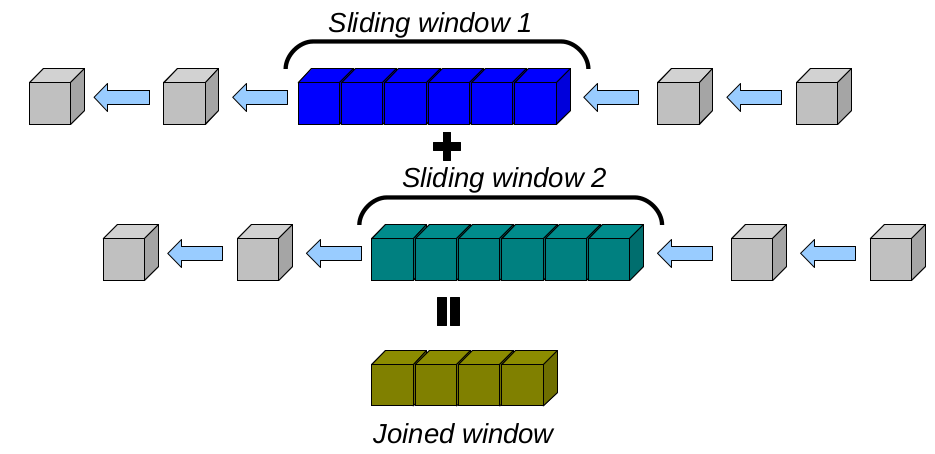
\includegraphics[scale=0.36]{img/drools-slide-00}
    
\end{figure}

Um nun, wie in Abschnitt \ref{szenario} beschrieben, einen erfolgreichen SSH Brute-Force 
Angriff zu erkennen, muss zuerst eine Brute-Force-Attacke erkannt werden, dazu dient die 
Regel \texttt{SSH brute-force attempt} (Anhang: \ref{app:drools-warning}). Die Regel 
untersucht nur Syslog-Meldungen die mit dem \textit{syslog-tag} \texttt{SSHFAILURE} 
versehen wurden. Es wird ein Event ausgelöst, wenn innerhalb von einer Minute vom 
gleichen Quell-Host und dessen verwendeten Benutzernamen 10 oder mehr fehlgeschlagene 
Login-versuche erfolgen. Als Event wird in diesem Fall eine neue Syslog-Meldung verfasst 
und mit dem Schweregrad \texttt{WARNING} und dem \textit{syslog-tag} \texttt{BRUTEFORCE} 
versehen. Die Meldung kann zum Beispiel persistent gespeichert werden (mehr dazu in 
Abschnitt \ref{nosql}) und an einen Monitor weitergeleitet werden.\\

Zur Erkennung einer erfolgreichen SSH Brute-Force-Attacke existiert ebenfalls eine 
beispielhafte Regel (Anhang: \ref{app:drools-emergency}). Die Regel \texttt{Successful 
SSH brute-force attack} löst einen Event aus, wenn innerhalb von 10 Sekunden nach dem 
Auftreten von Meldungen mit dem \textit{syslog-tag} \texttt{BRUTEFORCE} und 
\texttt{SSHFAILURE} und des zugehörigen Host und der verwendeten Benutzernamen, eine 
Meldung mit dem \textit{syslog-tag} \texttt{SSHSUCCSESS} auftritt, welche vom 
gleichen Host und aus der dazugehörigen Menge der Benutzernamen stammt.
Die generierte Syslog-Meldung wird mit dem gewichtigsten Schweregrad \texttt{EMERGENCY} 
und dem \textit{syslog-tag} \texttt{INCIDENT} markiert.\\

Mit diesem beiden Regeln ist es \textit{JCorrelat} unter der Zuhilfenahme von 
\textit{Drools-Fusion} möglich den einen Erfolgreichen Login unter tausenden 
Loginversuchen innerhalb einer Brute-Force-Attacke zu identifizieren.

\subsection{persistente Speicherung}\label{nosql}

In diesem Abschnitt wird Punkt \textbf{4} aus Abbildung \ref{pic:jcorrelat} erläutert.\\

Neben der direkten Alarmierung von IT-Sicherheitskritischen Ereignissen, ist ein weiteres 
Ziel der IT-Sicherheit die Verfügbarkeit der älterer Ereignisse um auch über längere 
Zeiträume hinweg verbindlich Auskunft über den Zustand eines Systems zu geben, oder die 
Daten mit neuen Methoden zu analysieren. Jedoch stellt die Speicherung von einer großen 
Menge sich ändernder Daten eine große Herausforderung dar. Mit \textit{JCorrelat} ist es 
möglich eine Vielzahl an Diensten zu überwachen, dabei können sich die zu betrachtenden 
Daten ständig ändern und es können Dienste hinzukommen oder wegfallen.\\

Eine erster Ansatz wäre die Speicherung der normalisierten Daten (Abschnitt 
\ref{syslog-konsolidierung}) in einer relationalen Datenbank. Aufgrund der dynamischen 
Natur der Daten müsste für eine effiziente Verarbeitung das Schema einer solchen 
Datenbank stetig angepasst werden, dieser Aufwand ist enorm und nicht Zielführend.\\
Im Gegensatz zum relationalen Ansatz wird bei \textit{NoSQL}-Datenbanken (Not only SQL) 
kein, oder nur ein minimales Schema gespeichert. Somit erlaubt dieses Konzept zu jeder 
Zeit eine Änderung der Struktur der Daten. Darüber hinaus lassen sich 
\textit{NoSQL}-Datenbanken über viele Instanzen hinweg skalieren und liefern Daten sehr 
schnell aus. Allerdings mit den Nachteil, dass nicht auf allen Systemen zeitgleich die 
aktuellsten Daten zur Verfügung stehen.\\

Grundsätzlich lassen sich drei Konzepte von \textit{NoSQL}-Datenbanken identifizieren. 
Zuerst sind die einfachen \textbf{\emph{key-value}}-Implementierungen zu nennen, diese 
Datenbanken sind mit Abstand die schnellsten, da die Werte lediglich ein \textit{BLOB} 
(Binary Large OBject) abgespeichert werden und somit nicht interpretiert werden. Damit 
sind die Werte nicht durchsuchbar, umso einfache ist dafür die API.\\

Die \textbf{\emph{column-oriented data stores}}-Lösungen speichern die Daten in Tabellen, 
ähnlich wie relationale-Lösungen, jedoch werden die Zeilen einer Tabelle in sogenannte 
shards (Scherben) unterteilt und die Spalten in Spaltengruppen, jeweils Abhängig von 
ihrem Schlüssel. Damit ist das Tabellenschema beliebig erweiterbar, aber eine 
Volltextsuche bietet diese Lösung nicht.\\

Davon abweichend arbeiten die \textbf{\emph{document-based data stores}}, sie speichern 
die Daten in \textit{documents} ab, welche eine Menge an beliebigen Argumenten mit einer 
unterschiedlichen Anzahl an Attributen beschreiben. Neue Objekte dürfen jederzeit neu 
angelegt werden und die Art und Anzahl ihrer \textit{key-value}-Paare ist nicht von 
Interesse. Als größter Vorteil ist hier die Möglichkeit zur Volltextsuche zu nennen.\\

Eben aus diesen letztgenannten Gründen kommt bei \textit{JCorrelat} 
\textit{elasticsearch}\footnote{\url{https://www.elastic.co/products/elasticsearch}} zum 
Einsatz, was die Konzepte eines \textbf{\emph{document-based data stores}} umsetzt. 
\textit{JCorrelat} sendet die normalisierten und korrelierten Syslog-Meldungen direkt an 
\textit{elasticsearch} für eine persistente Speicherung. Monitorsing- und 
Visualisierungssysteme können nun periodisch auf diese Daten zugreifen und kritische 
Ereignisse melden und visualisieren. Eine rudimentäre Visualisierung des SSH Brute-Force 
-Szenarios wurde in \cite{reissmann} veröffentlicht (Abbildung \ref{pic:logvis}). 
Alternative Möglichkeiten zu Visualisierung werden in Abschnitt \ref{ausblick} erläutert. 

\begin{figure}[htbp]
    \caption{Einfache Visualisierung durch JCorrelat}
    \label{pic:logvis}\vspace{0.2cm}
    \centering
    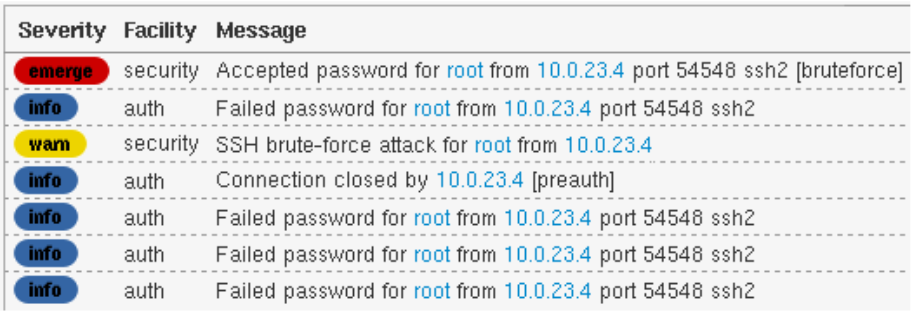
\includegraphics[scale=0.42]{img/correlat-ui}  
\end{figure}
\newpage
\subsection{Leistungsbetrachtung}\label{performance}

Wie schon in Sektion \ref{nosql} erwähnt, kostet das Korrelieren der Syslog-Meldungen am 
meisten Rechenzeit und ist daher der limitierende Faktor. Insbesondere stellt die 
Skalierbarkeit von \textit{Drools-Fusion} ein Problem dar, da es auf \textit{in memory 
engine} basiert, müssten mehrere Instanzen auf den gleichen Arbeitsspeicher zugreifen 
können (\textit{distributed memory}). Jedoch existieren laut \cite{reissmann} dafür keine 
Leistungsfähigen OpenSource-Lösungen, sodass eine Partitionierung nach Anwendung 
empfohlen wird. Somit ist nur eine \textit{JCorrelat}-Instanz für eine Anwendung 
zuständig. Es besteht ein Zusammenhang zwischen benötigten Arbeitsspeicher und der Größe 
des Betrachtungsfensters, benötigt eine Regel ein längeres Betrachtungsfenster umso mehr 
Meldungen müssen im Arbeitsspeicher gehalten werden.\\
Untersucht wird auch die Geschwindigkeit von \textit{rsyslog}, der ohne Normalisierung 
auf gängiger Hardware bei einer Syslog-Nachrichtengröße von 512 Byte über 200.000 
Syslog-Meldungen verarbeiten kann und damit die maximale Anzahl an Nachrichten auf einer 
1 GBit-Netzwerkschnittstelle verarbeiten kann.\\

Für den Benchmark wurden mithilfe der Software 
\textit{loggen}\footnote{\url{https://github.com/balabit/syslog-ng/blob/master/tests/loggen/loggen.md}}
 eine 20.000 Meldungen umfassende Datei in Dauerschleife  eingelesen und die daraus 
generierten Syslog-Meldungen an den Syslog-Server (Punkt \textbf{2} in Abbildung 
\ref{pic:jcorrelat}) weitergeleitet. Die Datei bestand zu circa einem Drittel aus 
SSH-Meldungen, der Rest waren andere übliche Syslog-Meldungen ohne Relevanz für die 
Korrelation.

\begin{figure}[htbp]
    \caption{Ergebnisse des Benchmark}
    \label{pic:benchmark}\vspace{0.2cm}
    \centering
    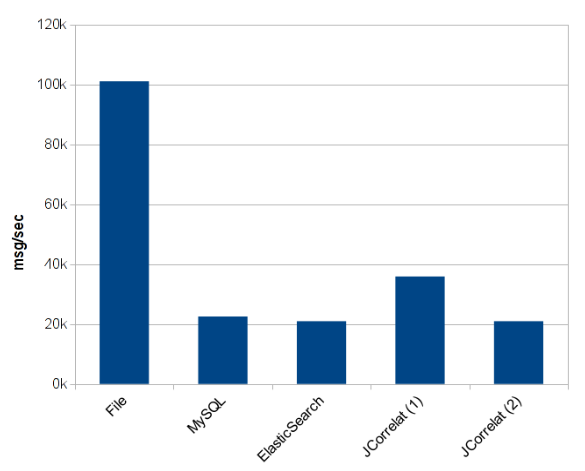
\includegraphics[scale=0.46]{img/benchmark}  
\end{figure}

Abbildung \ref{pic:benchmark} zeigt die Ergebnisse eines Benchmarks über das gesamte 
Korrelationssystem hinweg.\\

\textbf{File} zeigt die Anzahl der Meldungen nach der 
Normalisierung wenn diese einfach lokal in Dateien geschrieben werden.\\
Die Balken \textbf{Mysql} und \textbf{ElasticSearch} demonstrieren die Anzahl der 
normalisierten Syslog-Meldungen wenn diese direkt über \textit{rsyslog} eigene Module in 
diese Datenbanken geschrieben werden. Es wird eine auf HTTP-basierende API verwendet.\\
Über 30.000 normalisierte Syslog-Meldungen \textbf{JCorrelat (1)} können hingegen mit 
\textit{JCorrelat} über die \textit{elasticsearch}-API direkt in \textit{elasticsearch} 
geschrieben werden, was die Differenz zum vorhergehenden Balken erklärt, da hier der 
HTTP-Verwaltungsaufwand entfällt.\\
Bei \textbf{JCorrelat (2)} wurde auch die Korrelation aktiviert. Damit ist 
\textit{JCorrelat} nicht langsamer als wenn nur normalisierte Syslog-Meldungen in eine 
Datenbank geschrieben würden. 






 
%%%%%%%%%%%%%%%%%%%%%%%%%%%%%%%%%%%%%%%%%%%%%%%%%%%%%%%%%%%%%%%%%%%%%%%
\chapter{Auswertung und Visualisierung}\label{ausblick}
\thispagestyle{fancy}

Da \textit{JCorrelat} wohlformatierte Daten in \textit{elasticsearch} ablegt, ist es 
möglich mit einer Vielzahl an weiteren Werkzeugen diese Daten zu analysieren und zu 
visualisieren. Aus diesem Grund wurde auf der Basis von \cite{kleindienst} ein 
ELK-Stack aufgebaut um weitere beispielhafte Visualisierungen vorzustellen. Der 
Aufbau des verwendeten ELK-Stacks ist Schematisch in Abbildung \ref{app:demo-elk} (Anhang)
dargestellt. Für die Visualisierung zeigt sich die \textit{Kibana} verantwortlich.\\
Abbildung \ref{pic:elk-01} zeigt eine durch \textit{Kibana} erstellte Visualisierung, 
dabei \textit{Kibana} greift es auf Daten zurück, die durch \textit{Logstash} 
strukturiert in \textit{elasticsearch} abgelegt wurden.
Ähnlich wie im Beispielszenario, (Abschnitt \ref{szenario}) sind auch hier 
fehlgeschlagene SSH-Logins anschaulich gemacht. Die IP-Quelladressen wurden dabei 
mithilfe von \textit{Geotargeting} einer möglichen Region zugewiesen, ebenso die Anzahl 
der erfolglosen Loginversuche aus dieser Region über einen vorher definierten Zeitraum. 
Der Kreisdurchmesser hat keinerlei Bedeutung, lediglich der Farbverlauf gibt in fünf 
dynamisch errechneten Abstufungen die Anzahl der erfolglosen Versuche an, wie man am 
Beispiel Kiev deutlich sieht. Um auch alle Erfolgreichen Logins anzuzeigen ist eine 
weitere Karte notwendig (Abbildung \ref{pic:elk-02}).\\
Diese Form der Illustration würde sich auch für \textit{JCorrelat} anbieten, dann 
könnten die Ereignisse (Bruet-Force-Attacke und erfolgreicher Login während einer Attacke)
auf einer Karte darstellt werden.

\begin{figure}[htbp]
    \caption{Visualisierung mit Kibana (fehlgeschlagene Logins)}
    \label{pic:elk-01}\vspace{0.2cm}
    \centering
    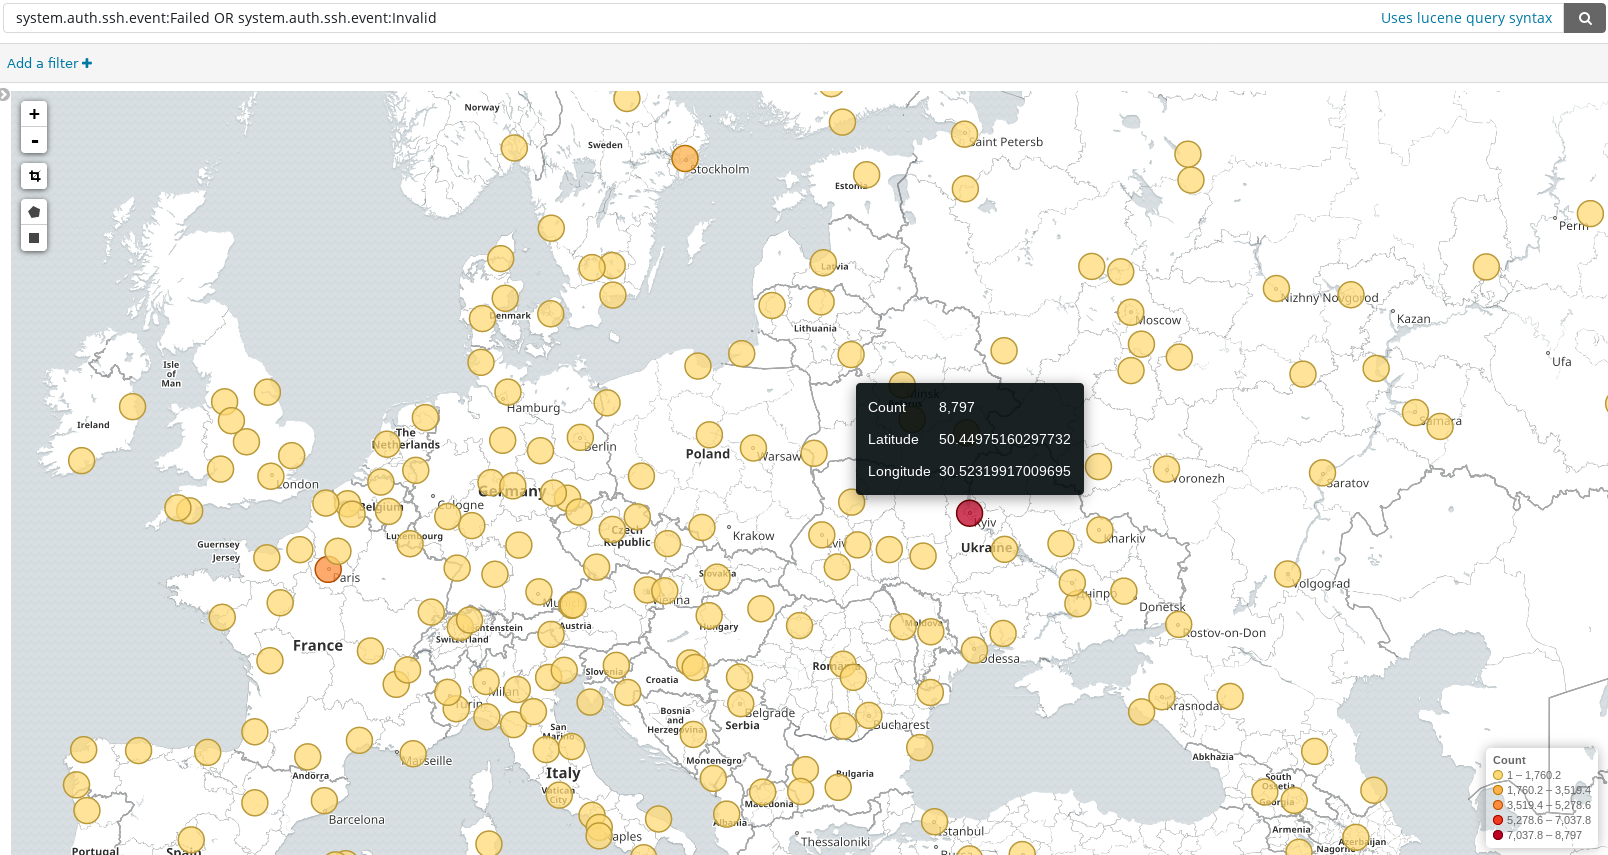
\includegraphics[scale=0.28]{img/elk-01}  
\end{figure}

\begin{figure}[htbp]
    \caption{Visualisierung mit Kibana (erfolgreiche Logins)}
    \label{pic:elk-02}\vspace{0.2cm}
    \centering
    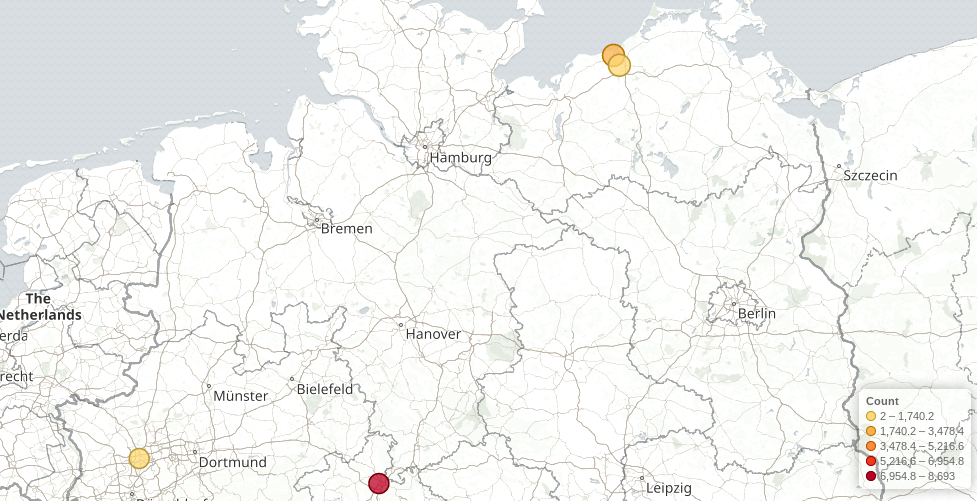
\includegraphics[scale=0.33]{img/elk-02}  
\end{figure}
%%%%%%%%%%%%%%%%%%%%%%%%%%%%%%%%%%%%%%%%%%%%%%%%%%%%%%%%%%%%%%%%%%%%%%%
\chapter{Fazit und Ausblick}
\thispagestyle{fancy}

Mit \textit{JCorrelat} wurde ein Prototyp für die automatische Korrelation und 
Konsolidierung von Syslog-Meldungen aus unterschiedlichen Quellen geschaffen. Wie die 
Ergebnisse des Benchmark zeigen skaliert der Prototyp sehr gut, wenn für jede Anwendung 
eine \textit{JCorrelat}-Instanz verwendet wird. Weniger Verwaltungsaufwand würde 
allerdings die Verwendung einer (eventuell auch proprietären) 
\textit{distributet-memory}-Lösung bieten, da dann die \textit{Drools-Fusion}-Regeln 
global platziert werden könnten und jede \textit{Drools}-Instanz auf den selben Daten 
arbeiten kann. Arbeitsspeicher ist auch der limitierende Faktor des Korrelationssystems, 
je mehr Arbeitsspeicher zur Verfügung steht umso mehr und größere Betrachtungsfenster 
kann \textit{Drools-Fusion} verwenden und so bessere Ergebnisse erzielen.\\

Durch die Normalisierung der Syslog-Meldung wird eine sehr effiziente Verdichtung von 
Informationen erreicht und Redundanzen werden größtenteils eliminiert. Das führt, neben 
der damit verbundenen hohen Ausführungsgeschwindigkeit der Korrelation, auch zu einem 
stark reduzierten Speicherbedarf für die persistente Speicherung. Durch die Wahl die 
normalisierten und korrelierten Daten in \textit{elasticsearch} abzuspeichern, bieten 
sich vielfältige Möglichkeiten der Auswertung und Visualisierung an. So Könnten bereits 
bestehende Monitoringsysteme um Plugins erweitert werden, welche die durch 
\textit{JCorrelat} erstellten Ereignisse periodisch abfragen und alarmieren können.\\

Auch eine Korrelation von weiteren Daten ist realisierbar, so könnten die 
Syslog-Meldungen auch mit Geo-Daten angereichert werde. 
%%%%%%%%%%%%%%%%%%%%%%%%%%%%%%%%%%%%%%%%%%%%%%%%%%%%%%%%%%%%%%%%%%%%%%%
\setcounter{page}{3}
\pagenumbering{Roman}
%%%%%%%%%%%%%%%%%%%%%%%%%%%%%%%%%%%%%%%%%%%%%%%%%%%%%%%%%%%%%%%%%%%%%%%
\bibliography{bib/bibo.bib}{}
\bibliographystyle{unsrt}
\thispagestyle{fancy}
\addcontentsline{toc}{chapter}{Literaturverzeichnis}
%%%%%%%%%%%%%%%%%%%%%%%%%%%%%%%%%%%%%%%%%%%%%%%%%%%%%%%%%%%%%%%%%%%%%%%
%lot und lof auf einer Seite
\listoffigures
\begingroup
\let\clearpage\relax
\listoftables
\endgroup
\thispagestyle{fancy}
%lot und lof im Inhaltsverzeichnis
\addcontentsline{toc}{chapter}{Abbildungsverzeichnis}
\addcontentsline{toc}{chapter}{Tabellenverzeichnis}
%%%%%%%%%%%%%%%%%%%%%%%%%%%%%%%%%%%%%%%%%%%%%%%%%%%%%%%%%%%%%%%%%%%%%%%
\chapter*{Anhang}\label{appendix}
\addcontentsline{toc}{chapter}{Anhang}
\thispagestyle{fancy}
\vspace{1cm}
\begin{figure}[htbp]
    \caption{Statusverlauf visualisiert mit \textit{NagVis}}
    \label{app:nag}\vspace{0.2cm}
    \centering
    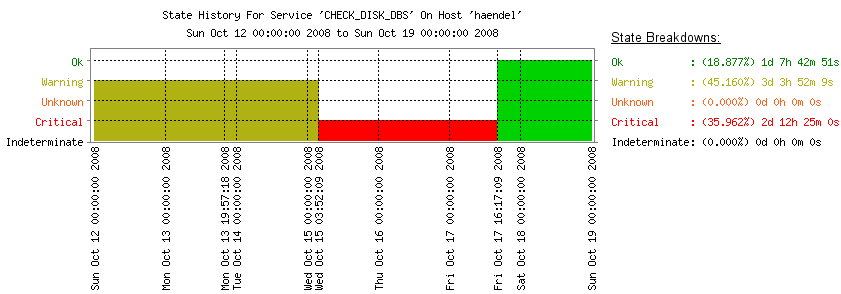
\includegraphics[scale=0.5]{img/nag_trend}  
\end{figure}

\vspace{4cm}
\begin{figure}[h]
    \caption{\textit{liblognorm} - Regel}
    \label{app:liblognorm-rule}\vspace{0.2cm}
    \centering
\begin{minipage}{0.8\textwidth}
\begin{minted}[mathescape,bgcolor=shadecolor]{perl6}
rule=SSHSUCCESS : Accepted password for %user:
word% from %ip:ipv4% port %port : number% %protocol:word%

rule=SSHFAILURE : Failed password for %user:
word% from %ip:ipv4% port %port : number% %protocol:word%

rule=SSHFAILURE : Failed password for invalid user %user:
word% from %ip:ipv4% port %port : number% %protocol:word%

\end{minted}
\end{minipage}
\end{figure}


\begin{figure}[h]
    \caption{\textit{liblognorm} - strukturierte Daten (JSON)}
    \label{app:liblognorm-normalisation}\vspace{0.2cm}
    \centering
    \begin{minipage}{0.8\textwidth}
\begin{minted}[mathescape,bgcolor=shadecolor]{json}
        
{   "data": {
        "protocol":"ssh2",
        "port" : "54548",
        "ip": "10.0.23.4",
        "user": "root"
    },
    "time":"2014-01-29T16:06:00.000",
    "host":"test.example.com",
    "facility":"auth",
    "severity":"info",
    "program" :"sshd",
    "message":" Failed password for root from
                10.0.23.4 port 54548 ssh2",
    "tags" : ["SSHFAILURE"] }
\end{minted}
\end{minipage}
\end{figure}


\begin{figure}[h]
    \caption{\textit{Drools} Brute Force - Regel}
    \label{app:drools-warning}\vspace{0.2cm}
    \centering
    \begin{minipage}{0.8\textwidth}
\begin{minted}[mathescape,bgcolor=shadecolor]{java}
        rule "SSH brute-force attempt"
        no-loop
        when
            Message (   $host:host,
                        $user:data["user"])
            $atts: CopyOnWriteArrayList(size >= 10)
                from collect(
                    Message(    tags contains"SSHFAILURE",
                                host == $host,
                                data["user" ] == $user)
                    over window : time (1m))
        then
            Message last = (Message) $atts.get($atts.size( )-1) ;
        
            for (Object f: $atts) {
                retract ( f ) ;
        }
        
            insert (messageFactory(last)
                . setTime(last.getTime( ))
                . setSeverity(Message.Severity.WARNING)
                . setFacility(Message.Facility.SECURITY)
                . setMessage("SSH brute-force attack" +
                    "for @{data.user} from @{data.ip}")
                . addTag ("BRUTEFORCE")
                . message( )) ;
        end        
        
\end{minted}
\end{minipage}
\end{figure}

\begin{figure}[h]
    \caption{\textit{Drools} - login detection Regel}
    \label{app:drools-emergency}\vspace{0.2cm}
    \centering
    \begin{minipage}{0.8\textwidth}
\begin{minted}[mathescape,bgcolor=shadecolor]{java}
       rule "Successful SSH brute-force attack"
       no-loop
       when
            $ att: Message (    tags contains "SSHFAILURE",
                                tags contains "BRUTEFORCE",
                                $host: host ,
                                $user: data ["user"])
            $ suc: Message (    host == $host,
                                data ["user" ] == $user,
                                tags contains "SSHSUCCESS",
                                this finishes[10 s] $att)
       then
            $att.addTag("INCIDENT");
            $att.setSeverity(Severity.EMERGENCY);
            $att.setMessage($att.getMessage( ) + "[bruteforce]");
       update ($att);
       end
        
\end{minted}
\end{minipage}
\end{figure}

\begin{figure}[htbp]
    \caption{Aufbau des verwendeten ELK-Stacks}
    \label{app:demo-elk}\vspace{0.2cm}
    \centering
    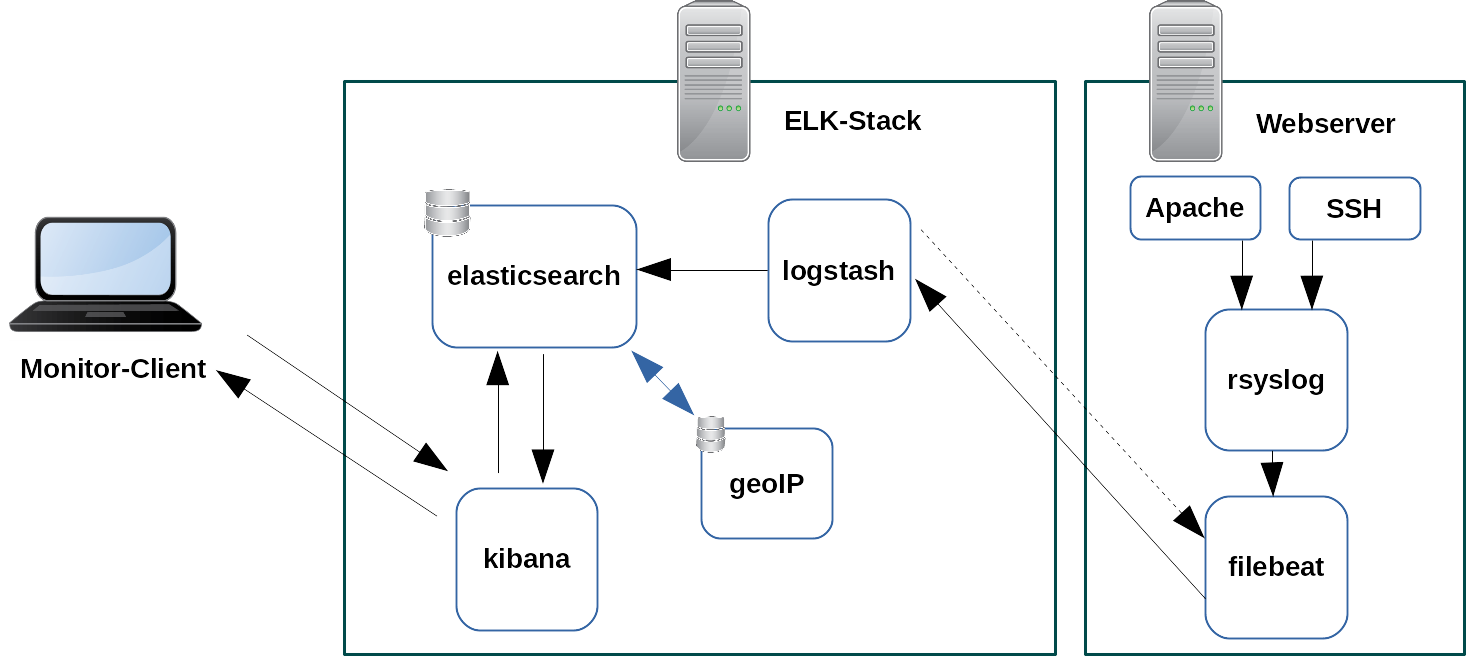
\includegraphics[scale=0.33]{img/demo-elk}  
\end{figure}

\end{document}
